\documentclass{beamer}
	
	\mode<presentation>
	{
		\usetheme{Madrid}
		\usecolortheme{default}
		\usefonttheme{serif}
		\setbeamertemplate{navigation symbols}{}
		\setbeamertemplate{caption}[numbered]
	
	\makeatother
	\setbeamertemplate{footline}
	{
	  \leavevmode%
	  \hbox{%
	  \begin{beamercolorbox}[wd=.4\paperwidth,ht=2.25ex,dp=1ex,center]{author in head/foot}%
	    \usebeamerfont{author in head/foot}\insertshortauthor
	  \end{beamercolorbox}%
	  \begin{beamercolorbox}[wd=.6\paperwidth,ht=2.25ex,dp=1ex,center]{title in head/foot}%
	    \usebeamerfont{title in head/foot}\insertshorttitle\hspace*{16em}
	    \insertframenumber{} / \inserttotalframenumber\hspace*{1ex}
	  \end{beamercolorbox}}%
	  \vskip0pt%
	}
	\makeatletter
	
	}
	
	\usepackage[french]{babel}
	\usepackage[utf8x]{inputenc}
	\usepackage{comment}
	\usepackage{graphicx}
	
	\newcommand{\colorized}[1]{{\color{red}{#1}}}
	
	
	% Presentation informations
	\title{Sécurité Web et audit}
	\author{Pierre-Marie JUNGES, Florent NOSARI}
	\institute[UL] {
		Université de Lorraine \\
	}
	
	\date{\today}
	
	\begin{document}
	
	\setbeamertemplate{headline}{}
	  \begin{frame}
	  	\titlepage 
	  \end{frame}
	
	\begin{frame}{Introduction}
		\begin{itemize}
			\item Audit de Sécurité
			\item +
			\item Sécurité Web
			\item = 
			\item Audit de sécurité d'une application web
		\end{itemize}
	\end{frame}
	
	\begin{frame}{Plan}
		\tableofcontents
	\end{frame}
	
	
	\section{Initier l'audit}
	
		\subsection{Termes et definitions}
		\begin{frame}{Termes et definitions}
			Audit:
			\begin{itemize}
				\setlength{\itemindent}{+.2in}
				\item Vue à un instant T de la sécurité d'un système
				\item Pratique encadré légalement (accord avec l'audité)
				\item Comparaison à un référentiel (loi, politique interne, références)
				\item Action ponctuelle
			\end{itemize}
			Auditeur:
					\begin{itemize}
						\setlength{\itemindent}{+.2in}
				\item Def
			\end{itemize}
			Audité:
					\begin{itemize}
						\setlength{\itemindent}{+.2in}
				\item Def
			\end{itemize}
		\end{frame}
	
	
		\subsection{Principes à respecter}
		\begin{frame}{Principes à respecter}
			\begin{enumerate}
				\item Intégrité
				\item Précision
				\item Professionnalisme
				\item Confidentialité
				\item Impartialité
				\item Approche factuelle
			\end{enumerate}
		
		\end{frame}
	
	
		\subsection{Mise en place}
		\begin{frame}{Mise en place}
		     Contact avec l'audité (réunion) : 
			\begin{itemize}
				\item Objectif
				\item Porté
				\item Méthodes (boite blanche/grise/noire)
				\item Composition de l'équipe
				\item Demandes techniques et administratives
				\item Définition des échéances
				\item Confirmation légale
			\end{itemize}		
		\end{frame}
	
		\begin{frame}{Mise en place}
			Contact avec l'audité (réunion) : 
			\begin{itemize}
				\item Objectif \colorized{Garantir une application sans failles de l'OWASP Top 10}
				\item Porté \colorized{Application web}
				\item Méthodes \colorized{Boite blanche}
				\item Composition de l'équipe
				\item Demandes techniques et administratives \colorized{code source}
				\item Définition des échéances \colorized{\today}
				\item Confirmation légale
			\end{itemize}		
		\end{frame}
	
		\begin{frame}{Mise en place}
			\begin{block}{OWASP Top 10 2017}
				\begin{enumerate}
					\item Injection
					\item Violation de gestion d'authentification et de session
					\item Cross-Site Scripting (XSS)
					\item Violation de contrôle d'accès
					\item Mauvaise configuration de sécurité
					\item Exposition de données sensibles
					\item Protection insufisante contre les attaques
					\item Falsification de requête intersites (CSRF)
					\item Utilisation de composants avec des vulnérabilités connues
					\item APIs non-sécurisée
				\end{enumerate}
			\end{block}
		\end{frame}
		
		\begin{frame}{Mise en place}
			Contact avec l'audité (réunion) : 
			\begin{itemize}
				\item Objectif \colorized{Garantir une application sans failles de l'OWASP Top 10}
				\item Porté \colorized{Application web}
				\item Méthodes \colorized{Boite blanche}
				\item Composition de l'équipe
				\item Demandes techniques et administratives \colorized{code source}
				\item Définition des échéances \colorized{\today}
				\item Confirmation légale
			\end{itemize}		
		\end{frame}
		
	\section{Execution de l'audit}	
		\subsection{Différentes pratiques}
			\begin{frame}{Différentes pratiques}
				Différentes pratiques existent : 
				\begin{itemize}
					\item Audit organisationnel
					\item Tests d'intrusion (fuzzing)				
					\item Revue de code source
					\item Relevés de configuration
					\item Analyse d'architecture	
				\end{itemize}		
			\end{frame}
		
			\begin{frame}{Différentes pratiques}
				Différentes pratiques existent : 
				\begin{itemize}
					\item Audit organisationnel
					\item \colorized{Tests d'intrusion (fuzzing)}
					\item \colorized{Revue de code source}
					\item \colorized{Relevés de configuration}
					\item Analyse d'architecture
				\end{itemize}		
			\end{frame}
		
		\subsection{Tests d'intrusion} 
			\begin{frame}{Outils utilisés}
				\begin{figure}
			        \centering
			        \begin{minipage}{.5\textwidth}
			            \centering
			            
\includegraphics[width=.4\linewidth]{schemas/images/metasploit.png}
			            \break
			            Metasploit
			        \end{minipage}%
			        \begin{minipage}{.5\textwidth}
			            \centering
			            
\includegraphics[width=.4\linewidth]{schemas/images/zap.png}
			            \break 
			            OWASP Zap
			        \end{minipage}
			    	%cerveau libre de droit
	    		\end{figure}	
			\end{frame}
			
			\begin{frame}{Injection - Principe}
					\begin{figure}
						\centering
						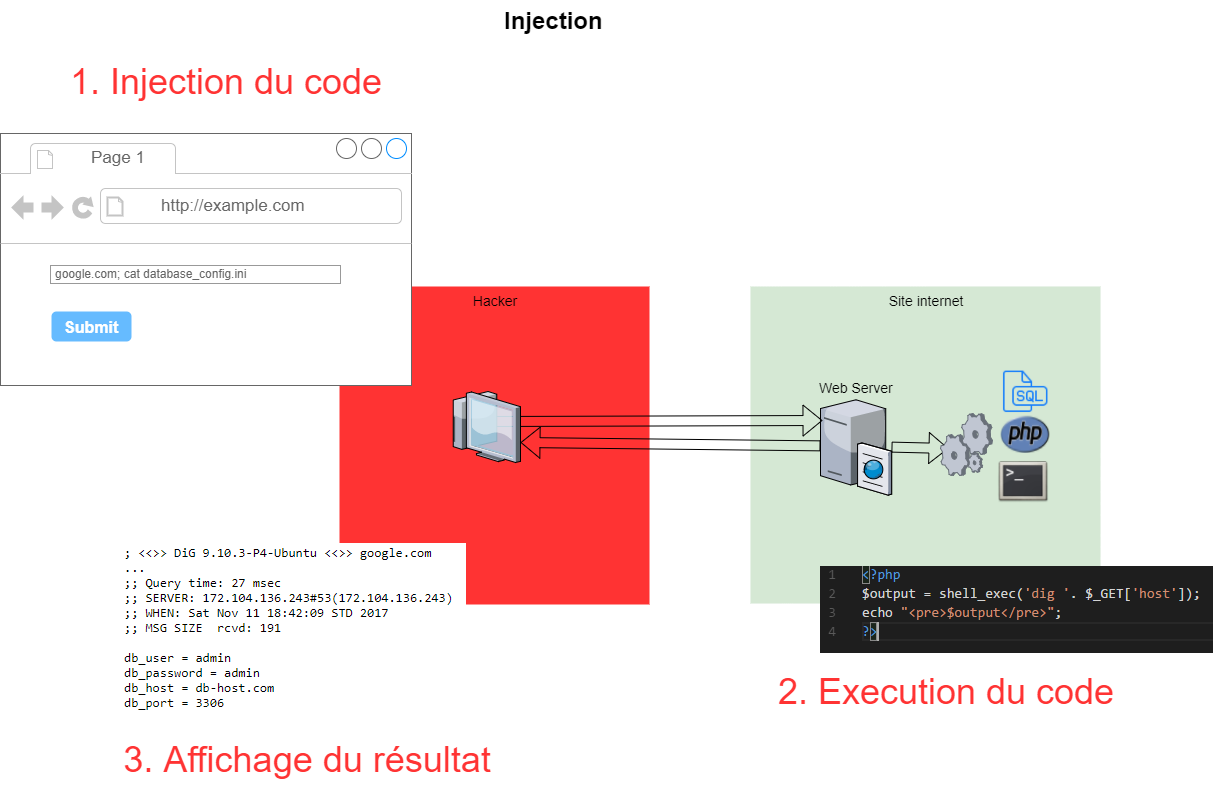
\includegraphics[width=0.9\linewidth]{schemas/images/injection.png}
						\caption{Déroulement d'une attaque}
					\end{figure}
			\end{frame}
		
			\begin{frame}{Injection - Démonstration}
			
			\end{frame}
	
			\begin{frame}{Violation de gestion d'authentification et de session - Principe}
			\begin{figure}
					\centering
					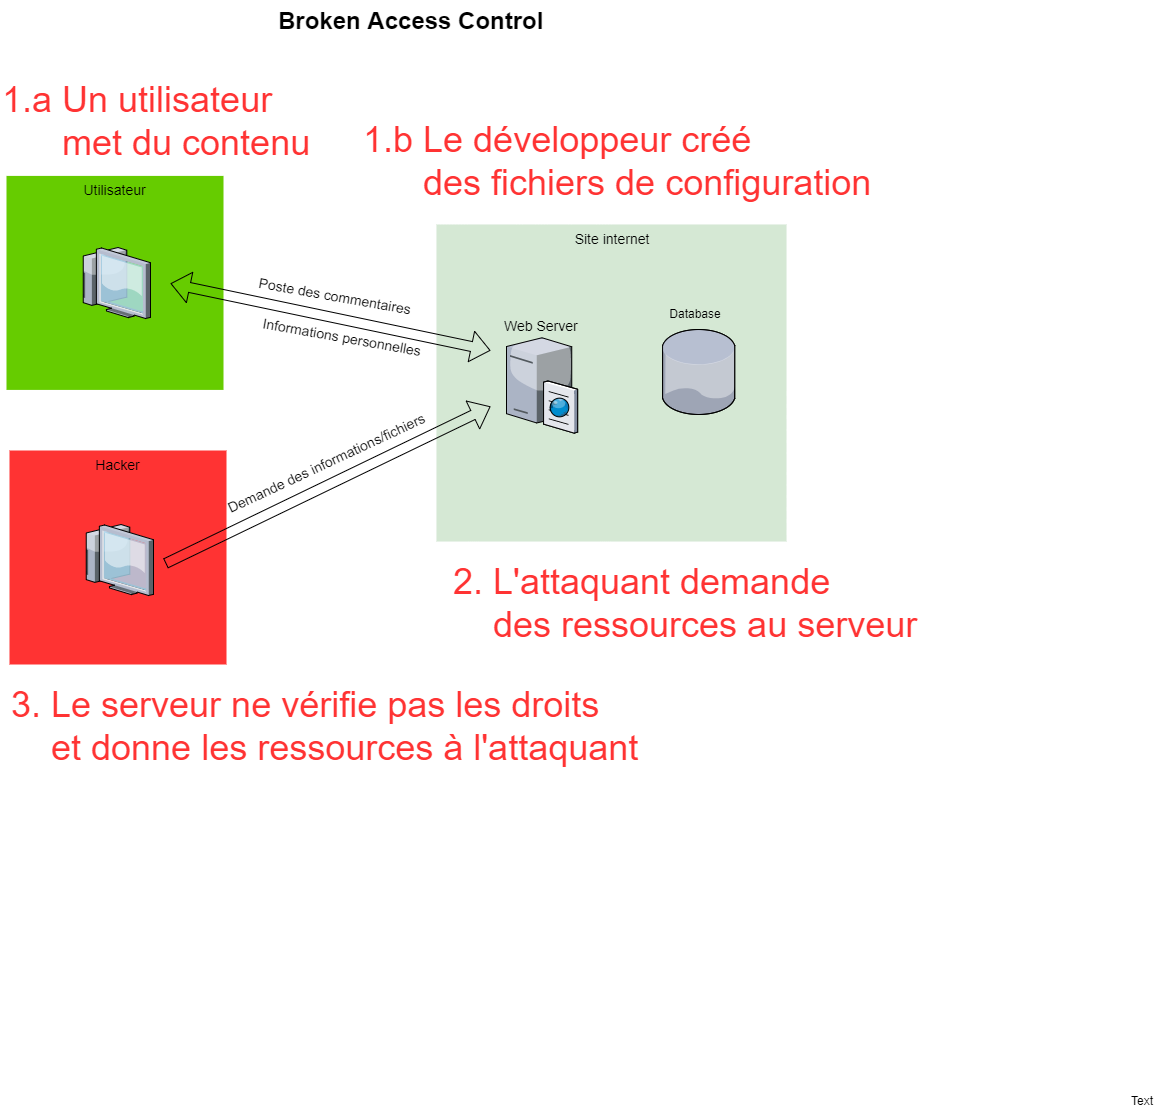
\includegraphics[width=0.9\linewidth]{schemas/images/broken_ac.png}
					\caption{Déroulement d'une attaque}
				\end{figure}
			\end{frame}
			
			\begin{frame}{Violation de gestion d'authentification et de session - Démonstration}
			
			\end{frame}
		
			\begin{frame}{Cross-Site Scripting (XSS) - Principe}
			\begin{figure}
					\centering
					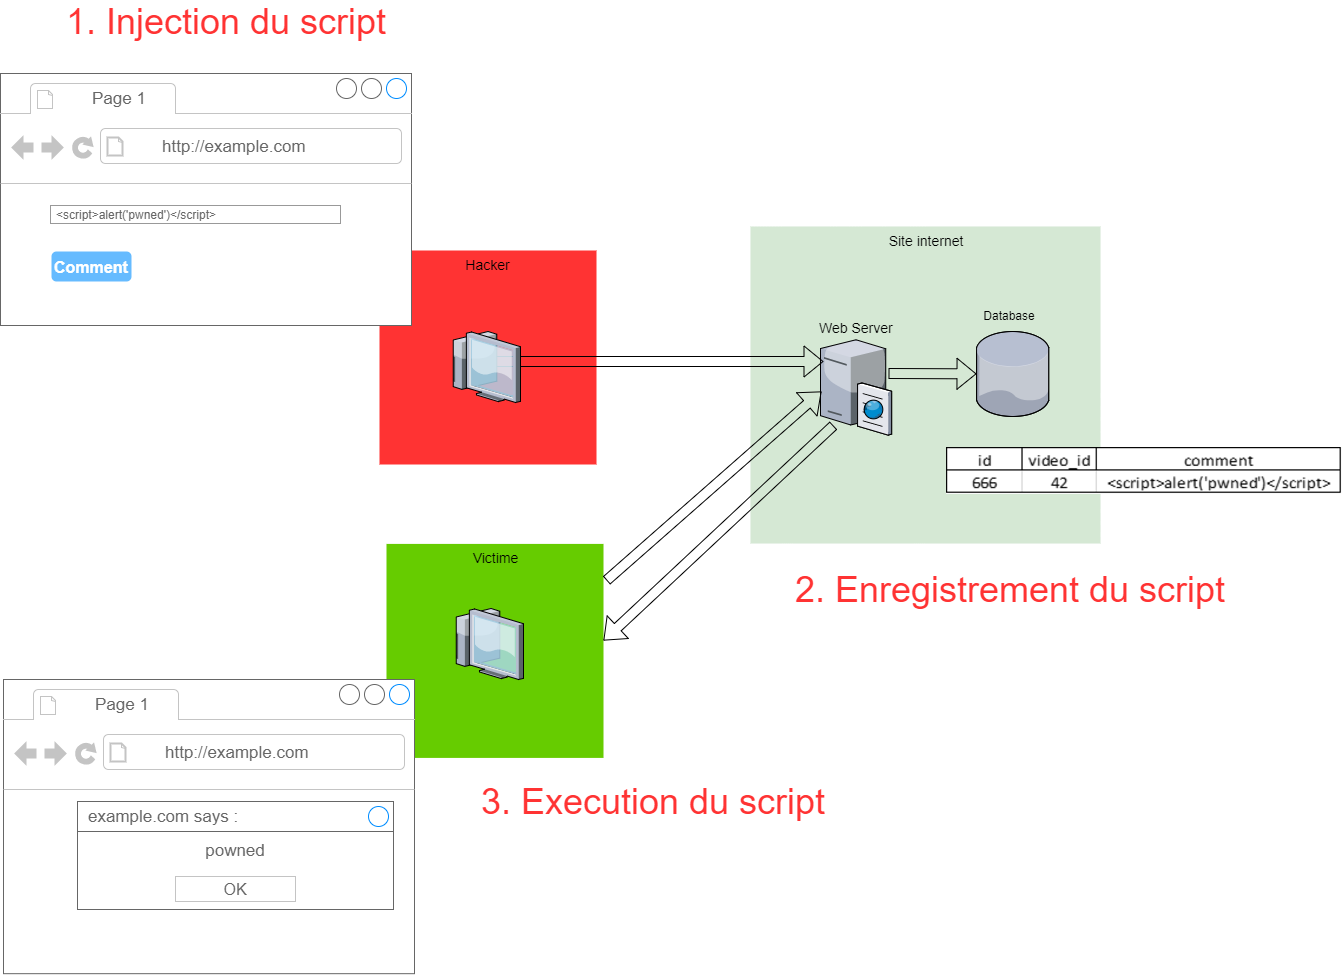
\includegraphics[width=0.9\linewidth]{schemas/images/XSS.png}
					\caption{Déroulement d'une attaque}
				\end{figure}
			\end{frame}
			
			\begin{frame}{Cross-Site Scripting (XSS) - Démonstration}
			
			\end{frame}
		
	\subsection{Tests d'intrusion} 
		\begin{frame}{Outils utilisés}
		\begin{figure}
			\centering
			\begin{minipage}{.5\textwidth}
				\centering
				
\includegraphics[width=.4\linewidth]{schemas/images/metasploit.png}
				\break
				Revue de code source
			\end{minipage}%
			
			%cerveau libre de droit
		\end{figure}	
		\end{frame}		
		
	\end{document}}